% Load before IEEEtran to avoid XeTeX TU/Times font substitutions.
\RequirePackage[T1]{fontenc}
\documentclass[conference,a4paper]{IEEEtran}
\IEEEoverridecommandlockouts

% Packages retained from the manuscript; duplicate/conflicting imports removed.
\usepackage{cite}
\usepackage{float}
\usepackage{amsmath,amssymb,amsfonts}
\usepackage{mathtools}
\usepackage{algorithm}
\usepackage{algpseudocode}
\usepackage{graphicx}
\usepackage{textcomp}
\usepackage{xcolor}
\usepackage{booktabs}
\usepackage{tabularx}
\usepackage{array}
\usepackage{nicematrix}
\usepackage{balance}
\usepackage{enumitem}
\usepackage{tikz}
\usepackage{bm}
\usepackage{lipsum}
\usetikzlibrary{shapes.geometric}
\usepackage[hidelinks]{hyperref}

\algrenewcommand\algorithmicrequire{\textbf{Input:}}
\algrenewcommand\algorithmicensure{\textbf{Output:}}
\newtheorem{coro}{Corollary}
\newtheorem{theo}{Theorem}
\newtheorem{prop}{Proposition}
\newtheorem{remark}{Remark}
\newtheorem{example}{Example}
\newtheorem{lemma}{Lemma}
\newtheorem{defin}{Definition}
\hypersetup{breaklinks=true,citecolor=black,colorlinks=true,
            linkcolor=black,urlcolor=blue}
\setcounter{MaxMatrixCols}{30}

\title{Mobility-Aware UAV Positioning and Secret Key Rate Optimization for HAP--UAV CV-QKD}
\author{\IEEEauthorblockN{TBD\IEEEauthorrefmark{1},
TBD\IEEEauthorrefmark{2}}
\IEEEauthorblockA{\IEEEauthorrefmark{1}XXX}
\IEEEauthorblockA{\IEEEauthorrefmark{2}Computer Communications Laboratory,
The University of Aizu, Aizuwakamatsu 965-8580, Japan}}


\begin{document}
\maketitle
\begin{abstract}
This provisional internal-review study examines source selection and UAV positioning for a cloud-affected HAP--UAV discrete-modulated CV-QKD model. A finite catalog of 233 exact-source ensembles defines a common location-dependent numerical rate map. An offline stationary benchmark, a current-slot Greedy policy, and finite-horizon dynamic programming (DP) are compared under identical cloud realizations and speed constraints. Across 100 paired missions, expanding the candidate set from 10 to 100 raises the mean DP penalized objective by 11.41\%. At blockage probability 0.8, mean zero-rate unavailability is 24.60\%, 16.53\%, and 4.07\% for Stationary, Greedy, and DP, respectively. At the representative penalty, DP reduces travel by 88.37\% relative to zero penalty while reducing mean usable rate by 0.515\%. These are conditional manuscript-model outputs: the recorded two-dimensional mutual information and homodyne Holevo expression do not specify a consistent Bob measurement. The results characterize the saved numerical optimization and do not establish physical quantum security.
\end{abstract}
\begin{IEEEkeywords}
Continuous-variable quantum key distribution, UAV, high-altitude platform, cloud blockage, probabilistic shaping, dynamic programming.
\end{IEEEkeywords}
\noindent\textbf{Internal review only.} Security-model correction and author review remain pending. Status:\\
{\footnotesize\texttt{UNVALIDATED\_SECURITY\_MODEL};}\\
{\footnotesize\texttt{NOT\_READY\_FOR\_PUBLICATION\_SCALE\_RUNS}.}
\typeout{COMPACT_LAYOUT textheight=\the\textheight;columnwidth=\the\columnwidth;textwidth=\the\textwidth;topmargin=\the\topmargin;headheight=\the\headheight;headsep=\the\headsep;voffset=\the\voffset}
\section{HAP--UAV CV-QKD System and Problem Formulation}
\label{sec:system}
\subsection{Mobility-Aware UAV Positioning and SKR Optimization}
We consider one UAV at a fixed altitude over a $1\,\mathrm{km}\times
1\,\mathrm{km}$ area, discretized into $J$ candidate positions
$\mathcal Q=\{\mathbf q_j\}_{j=1}^J$. The mission has $N_t$ slots of
duration $\Delta t$. Let $c_{j,n}\in\{0,1\}$ indicate cloud blockage
(one means blocked). The matrix $\mathbf C=[c_{j,n}]$ contains spatially
and temporally correlated Bernoulli states. P2 and P3 know the complete
matrix and are offline benchmarks; Greedy observes only the current slot.

For an unblocked link, the recorded manuscript-style raw rate is
\begin{equation}
 K_j(\nu,V_A)=\beta_{\rm rec}I_{AB,j}^{2D}(\nu,V_A)-\chi_{BE,j}(\nu,V_A).
 \label{eq:raw}
\end{equation}
Equation~\eqref{eq:raw} is retained as a conditional numerical metric,
subject to the measurement-consistency limitations below.

\subsection{Recorded Physical-Layer Model and Security Boundary}
\label{sec:security}
Alice sends the coherent-state ensemble $\{p_k,\alpha_k\}_{k=1}^{256}$.
With $[\hat x,\hat p]=2i$ and vacuum quadrature variance one, the
normalization is $V_A=2\sum_kp_k|\alpha_k|^2=2\bar n$.
The source moments $C_s,w_s$ are computed from this same ensemble;
the subscript distinguishes them from the cloud matrix.
For clear-sky power transmittance $\eta$, the saved evaluator uses
\begin{align*}
 \eta_f&=\langle\sqrt\eta\rangle^2,\\
 N=\eta_f\xi_f&=(\langle\eta\rangle-\eta_f)V_A
                  +\xi_{\rm ch}\langle\eta\rangle,\\
 V&=1+V_A,\qquad W=1+\eta_fV_A+N,\\
 Z&=2\sqrt{\eta_f}C_s-\sqrt{2Nw_s}.
\end{align*}
The convention is $\xi_n=\xi_{\rm ch}$. The additive $N$ is
output-referred excess noise; loss-induced vacuum is already included
in $W$'s unit baseline. The active detector is ideal (efficiency one,
electronic noise zero). No imperfect trusted-detector claim is made.
The clear-sky distribution retains a separate angle-of-arrival outage
atom at $\eta=0$ and its active density on $[0,1]$, without renormalizing.
Moment reduction at the covariance level has a precedent for Gaussian
modulation~\cite{usenko2012}; it is not an identity for the full
discrete-input fading likelihood.

Specifically, the saved MI kernel uses the normalized likelihood
\[
 p_{\rm num}(\mathbf y|k)=\frac{
 \exp[-\|\mathbf y-2\sqrt{\eta_f}(\Re\alpha_k,\Im\alpha_k)\|^2/
                 (2(1+N))]}{2\pi(1+N)}
\]
and integrates both real components to obtain $I_{AB}^{2D}$.
The Holevo branch uses the standard-form covariance with entries
$V,W,Z$ and the \emph{homodyne} conditional eigenvalue
\[
 \nu_3^{\rm hom}=\sqrt{V(V-Z^2/W)}.
\]
These two branches do not specify one consistent single-mode Bob
measurement: a homodyne outcome has one quadrature, while joint
measurement of both quadratures adds measurement vacuum. The
measurement-dependent Holevo expressions are explicitly different
in~\cite{denys2021}. Consequently, all reported ``usable SKR'' values
are conditional outputs of the recorded manuscript model, not
established achievable secret-key rates.

Further, evaluating only $Z_-$ does not establish the worst-case
Holevo value over all admissible correlations; the general
interval-maximization caveat in~\cite[Sec.~4, footnotes 11--12]{denys2021}
also applies. A consistent measurement/noise specification, admissible
correlation treatment, parameter estimation, and fading/outage
conditioning protocol require author review. No correction is applied
to the historical numerical results in this manuscript revision.


\section{Optimization Problem}
\label{sec:optimization}
At each location, the finite exact-source catalog $\mathcal G$ contains
197 MB-shaped and 36 uniform 256-QAM ensembles. Searching the MB shaping
parameter $\nu$ and modulation variance $V_A$ gives
\begin{equation}
 \mathcal P_1:\quad K_j^\star=
 \left[\max_{(\nu,V_A)\in\mathcal G}K_j(\nu,V_A)\right]^+.
 \label{eq:p1}
\end{equation}
Each candidate uses its own authenticated source moments; the raw maximum
is selected before clipping. Channel moments independent of the source can
be shared, while the modulation-dependent fading noise is evaluated for
each $V_A$. The optimum is restricted to $\mathcal G$, rather than a
continuous shaping domain. With complete cloud blockage,
$S_{j,n}=(1-c_{j,n})K_j^\star$. Offline stationary selection is
\begin{equation}
 \mathcal P_2:\quad j_{\rm fix}^\star=
 \arg\max_j\frac{1}{N_t}\sum_{n=1}^{N_t}S_{j,n}.
 \label{eq:p2}
\end{equation}
The chosen location balances clear-sky rate and the full cloud sequence;
it need not be the location with the largest clear-sky rate alone.
For $j_n\in\{1,\ldots,J\}$ and
$d_{i,j}=\|\mathbf q_i-\mathbf q_j\|_2$, mobility optimization is
\begin{align}
 \mathcal P_3:\quad\max_{\{j_n\}}\quad&
 \underbrace{\frac{1}{N_t}\sum_{n=1}^{N_t}S_{j_n,n}}_{\overline K}
 -\frac{\lambda}{D_{\rm ref}}
 \underbrace{\sum_{n=2}^{N_t}d_{j_{n-1},j_n}}_{D}
 \label{eq:p3}\\
 \text{s.t.}\quad&d_{j_{n-1},j_n}\le v_{\max}\Delta t,\quad n\ge2.
 \nonumber
\end{align}
The objective is $U=\overline K-\lambda D/D_{\rm ref}$, with
$D_{\rm ref}>0$ and $\lambda\ge0$ in bit/use. Staying and a free initial
position are allowed; no terminal, deployment, or return requirement is
imposed. Distance is a mobility-cost surrogate, not propulsion energy.
\begin{figure*}[!t]
\centering
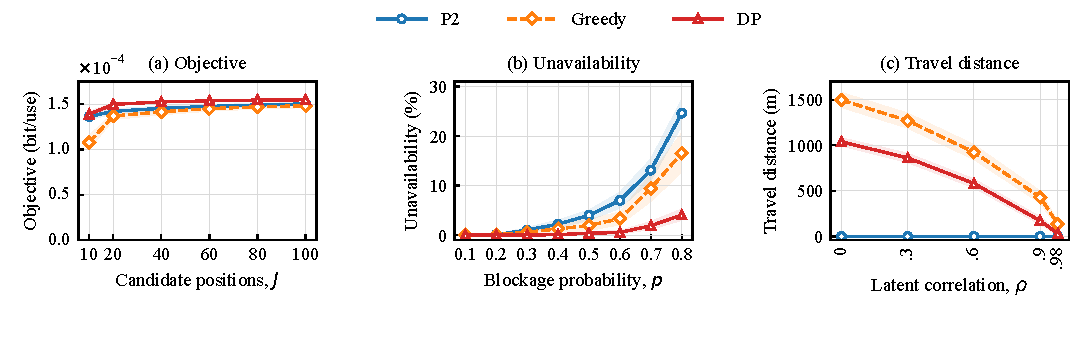
\includegraphics[width=\textwidth]{figures/compact_sensitivity.pdf}
\caption{Parameter sensitivity at $\lambda_{\rm ref}$: (a) objective versus
candidate count; (b) zero-SKR unavailability versus blockage probability;
(c) travel distance versus latent temporal correlation. Curves use 100 paired
missions; shaded bands are pointwise 95\% whole-mission bootstrap intervals.}
\label{fig:compact}
\end{figure*}

\section{Proposed Solution}
\label{sec:method}
P1 exhausts the finite catalog once per clear-sky position, reusing exact
source moments; P2 compares all full-horizon location means. For P3, let
$\mathcal N(j)=\{i:d_{i,j}\le v_{\max}\Delta t\}$. DP uses
\begin{align}
 F_1(j)&=S_{j,1},\label{eq:dp_init}\\
 F_n(j)&=S_{j,n}+\max_{i\in\mathcal N(j)}
 \left[F_{n-1}(i)-\frac{N_t\lambda}{D_{\rm ref}}d_{i,j}\right].
 \label{eq:dp}
\end{align}
Every feasible predecessor is considered, including staying, and the
retained state summarizes the best prefix ending at that location.
Backtracking saved predecessors from $\arg\max_jF_{N_t}(j)$ recovers the
finite-grid optimum, with $U^\star=\max_jF_{N_t}(j)/N_t$ and time
$O(N_tJ^2)$. Backpointers require $O(N_tJ)$ storage, in addition to the
$O(J^2)$ distance matrix. The stored implementation state $F_n/N_t$
has reward $S_{j,n}/N_t$ and edge cost $\lambda d_{i,j}/D_{\rm ref}$,
which is the same normalization. Both P2 and DP know the complete cloud sequence offline.
Greedy starts at $\arg\max_jS_{j,1}$, then maximizes the current-slot
score $S_{j,n}-N_t\lambda d_{j_{n-1},j}/D_{\rm ref}$ over feasible moves,
in $O(N_tJ)$ time. All methods share rates, clouds, and constraints.
DP dominates their penalized objectives, not necessarily each mission's
SKR or availability. Their difference also reflects DP's future-state and
initial-position information, so it does not measure an online control gain.
Without feasible movement, DP reduces to P2. P2 itself is independent of
the movement penalty because its path has zero distance.

\section{Numerical Results and Discussion}
\label{sec:numerical}
The synthetic HAP/UAV altitudes are 20/1 km; the $1\,\mathrm{km}^2$ grid
has 100 centers spaced 100 m apart. Missions have $30\times20$ s slots,
$v_{\max}=15$ m/s, and $D_{\rm ref}=1000$ m. The synthetic deployment
places the HAP horizontally at $(11419.6551,450)$ m and uses UAV
coordinates $50,150,\ldots,950$ m along each axis. Saved missions use
seed 20261015 and realization IDs 0--99. The retained optical settings
are 1550 nm, full divergence $233\,\mu$rad, receiver diameter 0.08 m,
$\beta_{\rm rec}=0.95$, $\xi_{\rm ch}=0.0186$ SNU, and ideal detection.
Saved Gaussian-copula complete-blockage clouds default to
$(p,\ell,\rho)=(0.4,250\,\mathrm m,0.9)$, with latent spatial covariance
$\Sigma_{ij}=\exp(-d_{i,j}/\ell)$ and a stationary AR(1) coefficient
$\rho$. Latent parameters differ from Bernoulli-cloud correlations.
Each latent state is thresholded at $\Phi^{-1}(p)$, where $\Phi$ is the
standard-normal distribution function; the marginal blockage probability
is prescribed, rather than measured meteorology.
We compare 100 paired missions
at fixed $\lambda_{\rm ref}=9.468026677248516\times10^{-6}$ bit/use.
Means and pointwise confidence intervals use independent whole missions,
not cells or slots; methods share each realization ID and configurations
use common innovations. No new physical-layer evaluation is required.
These intervals describe mission variability, rather than finite-key
parameter-estimation uncertainty or a quantum-security bound.
Availability means $S>0$, without an engineering threshold. In
Fig.~\ref{fig:compact}(a), expanding deterministic nested position sets
from $J=10$ to 100 raises mean DP $U$ by 11.409\% relative to $J=10$.
The improvement combines more spatial choices and greater connectivity;
optimal P2/DP objectives cannot decrease as the feasible set expands.
The comparative presentation follows~\cite{gong2020}.

At $p=0.8$, mean unavailability is 24.60\%, 16.53\%, and 4.07\% for
P2, Greedy, and DP, respectively [Fig.~\ref{fig:compact}(b)]. Cloud-aware
movement improves this observed metric, although P3 optimizes $U$.
Increasing $p$ under nested masks removes rewards, so optimal P2/DP
objectives cannot increase; no general availability ordering follows.
As latent $\rho$ increases from 0 to 0.98, DP distance decreases from
1038.25 to 31.84 m [Fig.~\ref{fig:compact}(c)], while its mean objective
gain over P2 decreases from 23.712\% to 0.155\%, relative to the
corresponding P2 mean. Persistent favorable locations make offline
stationary selection competitive. At the high-correlation endpoint, the
latent persistence time exceeds the mission horizon, allowing P2 to exploit
locations favorable throughout the mission. This is not a universal
monotonic law or a demonstration with forecast errors.

On the same default missions, changing DP from zero penalty to
$\lambda_{\rm ref}$ reduces mean distance by 88.370\% and mean usable
SKR by 0.515\%, relative to their respective zero-penalty means. Thus,
most movement can be avoided with a small numerical rate loss. P1
selects MB $(\nu,V_A)=(0.125,8)$ everywhere, at the MB catalog's variance
boundary; positioning gains do not isolate shaping gain. All rates remain
conditional outputs of the mixed 2D-MI/homodyne-Holevo model in
Section~\ref{sec:security}, without a validated quantum-security guarantee.
Finite-key estimation, key aggregation across fading states, tracking
interruptions, and reacquisition overhead are outside this comparison.
Trusted receiver imperfections would require a separate
model~\cite{usenko2016}.

\section{Conclusion}
\label{sec:conclusion}
Finite-catalog source selection, offline stationary positioning, and DP
trajectory optimization jointly characterize cloud-aware HAP--UAV
performance. Under the evaluated configurations, DP improves the
mobility-penalized objective over Stationary and Greedy, with observed
availability benefits. A distance penalty substantially reduces movement
while preserving most usable rate. Conclusions remain limited to a finite
grid, synthetic clouds, offline future information, and an uncalibrated
mobility-cost surrogate. The inconsistent MI/Holevo measurement pairing
requires correction before interpreting numerical rates as secure keys.

\bibliographystyle{IEEEtran}
\bibliography{manuscript_refs}
\end{document}
